
\chapter{Numerical and Physical Accuracy\label{chpt:accuracy}}

This chapter gives a systematic comparison between algorithms for
the evaluation of the excess free energy $\mathcal{F}_{\mathrm{exc}}$
and its gradient $\gamma$ in terms of accuracy. As the theory does
not contain any unpredictable random part, the comportment of the
code is mathematically predictable. For example, certain algorithms
should give the same result at machine precision ($10^{-13}$ to $10^{-15}$)
in certain conditions. A loss of accuracy comparing to the prediction
can be classified as two different types. One is the theoretical loss;
for instance, a certain equation is only valid for an infinite order.
This kind of loss is unavoidable but should be worked out explicitly.
Another source is the unknown loss, containing all kinds of incompatibility
in the result that cannot be explained mathematically. It is mainly attributable to a bug in the implementation that cannot be located. There is also the possibility that it is a theoretical loss which has not been worked out. All these comparisons aim to give a global view of the credibility for the results given by this code.

\section{Generalized spherical harmonics transform\label{sec:gsh-imp}}

As discussed in $\mathsection$\ref{sec:fgsht}, the function after
a forward-backward \acs{GSHT} process 
\begin{equation}
F_{\mu'\mu}^{m}=\frac{f_{m}}{8\pi^{2}}\sum_{i=0}^{m_{\mathrm{max}}}w_{i}\sum_{j=0}^{2m_{\mathrm{max}}}\sum_{k=0}^{2\left\lfloor m_{\mathrm{max}}/s\right\rfloor }F(\Theta_{i},\Phi_{j},\Psi_{k})R_{\mu'\mu}^{m*}(\Theta_{i},\Phi_{j},\Psi_{k})
\end{equation}
\begin{equation}
F(\Theta_{i},\Phi_{j},\Psi_{k})=\sum_{m=0}^{n_{\mathrm{max}}}f_{m}\sum_{\mu'=-m}^{m}\sum_{\underset{\mod(\mu,s)=0}{\mu=-m}}^{m}F_{\mu'\mu}^{m}R_{\mu'\mu}^{m}(\Theta_{i},\Phi_{j},\Psi_{k})
\end{equation}
only remains the same when it is a polynomial of both $\cos\Theta$,
$\cos\Phi$ and $\cos\Psi$ of order $n_{\max}$, where $n_{\max}$
is the highest order of \acs{GSH} in the expansion, and $m_{\max}=n_{\max}$
the order of quadrature used. However, as in reality, the density
variable $\rho$ is not a simple polynomial, and the choice of $m_{\max}$
and $n_{\max}$ is tightly linked to the performance. It is important
to know how much these choices will affect the results. The \acs{FFT}
process is implemented by package FFTW3 \citep{FFTW3}, which is verified
to be leading to strictly no accuracy lost (at machine precision).
That means the \acs{FGSHT} process will have strictly with the \acs{GSHT} %'will have strictly'? Something is missing.
process. Here we do not need to distinguish the two.

\subsection{$m_{\mathrm{max}}$ and $n_{\mathrm{max}}$ of projections}

The numerical error tests of a forward-backward GSHT process with
different order $n_{\mathrm{max}}$ of GSH and $m_{\mathrm{max}}$
of quadrature are shown in table \ref{tab:error-gsh}.
\begin{table}[H]
\begin{centering}
\subfloat[$f(\mathbf{\Omega})=1$]{\begin{centering}
\begin{tabular*}{1\columnwidth}{@{\extracolsep{\fill}}ccccccc}
\toprule 
{\footnotesize{}$m$\textbackslash{}$n$} & \multirow{1}{*}{{\footnotesize{}0}} & \multirow{1}{*}{{\footnotesize{}1}} & {\footnotesize{}2} & \multirow{1}{*}{{\footnotesize{}3}} & \multirow{1}{*}{{\footnotesize{}4}} & \multirow{1}{*}{{\footnotesize{}5}}\tabularnewline
\midrule
\multicolumn{1}{c}{{\footnotesize{}0}} & \textbf{\footnotesize{}0 (0)} & {\footnotesize{}9.00 (3.00)} & {\footnotesize{}34.00 (18.00)} & {\footnotesize{}83.00 (39.00)} & {\footnotesize{}164.00 (84.00)} & {\footnotesize{}285.00 (139.00)}\tabularnewline
\multicolumn{1}{c}{{\footnotesize{}1}} & \textbf{\footnotesize{}0 (0)} & \textbf{\footnotesize{}0 (0)} & {\footnotesize{}0 (1.67)} & {\footnotesize{}4.34 (6.07)} & {\footnotesize{}7.06 (13.63)} & {\footnotesize{}14.88 (17.30)}\tabularnewline
\multicolumn{1}{c}{{\footnotesize{}2}} & \textbf{\footnotesize{}0 (0)} & \textbf{\footnotesize{}0 (0)} & \textbf{\footnotesize{}0 (0)} & {\footnotesize{}0 (0)} & {\footnotesize{}0 (0)} & {\footnotesize{}5.65 (2.71)}\tabularnewline
{\footnotesize{}3} & \textbf{\footnotesize{}0 (0)} & \textbf{\footnotesize{}0 (0)} & \textbf{\footnotesize{}0 (0)} & \textbf{\footnotesize{}0 (0)} & {\footnotesize{}0 (0)} & {\footnotesize{}0 (0)}\tabularnewline
\multicolumn{1}{c}{{\footnotesize{}4}} & \textbf{\footnotesize{}0 (0)} & \textbf{\footnotesize{}0 (0)} & \textbf{\footnotesize{}0 (0)} & \textbf{\footnotesize{}0 (0)} & \textbf{\footnotesize{}0 (0)} & {\footnotesize{}0 (0)}\tabularnewline
\multicolumn{1}{c}{{\footnotesize{}5}} & \textbf{\footnotesize{}0 (0)} & \textbf{\footnotesize{}0 (0)} & \textbf{\footnotesize{}0 (0)} & \textbf{\footnotesize{}0 (0)} & \textbf{\footnotesize{}0 (0)} & \textbf{\footnotesize{}0 (0)}\tabularnewline
\bottomrule
\end{tabular*}
\par\end{centering}
}
\par\end{centering}
\begin{centering}
\subfloat[$f(\mathbf{\Omega})=\cos3\Theta$]{\begin{centering}
\begin{tabular*}{1\columnwidth}{@{\extracolsep{\fill}}ccccccc}
\toprule 
{\footnotesize{}$m$\textbackslash{}$n$} & \multirow{1}{*}{{\footnotesize{}0}} & \multirow{1}{*}{{\footnotesize{}1}} & {\footnotesize{}2} & \multirow{1}{*}{{\footnotesize{}3}} & \multirow{1}{*}{{\footnotesize{}4}} & \multirow{1}{*}{{\footnotesize{}5}}\tabularnewline
\midrule
\multicolumn{1}{c}{{\footnotesize{}0}} & {\footnotesize{}0 (0)} & {\footnotesize{}0 (0)} & {\footnotesize{}0 (0)} & {\footnotesize{}0 (0)} & {\footnotesize{}0 (0)} & {\footnotesize{}0 (0)}\tabularnewline
\multicolumn{1}{c}{{\footnotesize{}1}} & {\footnotesize{}0.96 (0.96)} & {\footnotesize{}0 (0)} & {\footnotesize{}0 (0)} & {\footnotesize{}2.56 (6.99)} & {\footnotesize{}10.76 (14.15)} & {\footnotesize{}13.83 (21.21)}\tabularnewline
\multicolumn{1}{c}{{\footnotesize{}2}} & {\footnotesize{}0.46 (0.46)} & {\footnotesize{}0 (0)} & {\footnotesize{}0 (0)} & {\footnotesize{}0 (0)} & {\footnotesize{}0 (0)} & {\footnotesize{}1.36 (0.50)}\tabularnewline
{\footnotesize{}3} & {\footnotesize{}0.86 (0.86)} & {\footnotesize{}0.66 (0.66)} & {\footnotesize{}0.66 (0.66)} & \textbf{\footnotesize{}0 (0)} & {\footnotesize{}0 (0)} & {\footnotesize{}0.66 (0.66)}\tabularnewline
\multicolumn{1}{c}{{\footnotesize{}4}} & {\footnotesize{}0.99 (0.99)} & {\footnotesize{}0.80 (0.80)} & {\footnotesize{}0.80 (0.80)} & \textbf{\footnotesize{}0 (0)} & \textbf{\footnotesize{}0 (0)} & {\footnotesize{}0 (0)}\tabularnewline
\multicolumn{1}{c}{{\footnotesize{}5}} & {\footnotesize{}0.83 (0.83)} & {\footnotesize{}1.01 (1.01)} & {\footnotesize{}1.01 (1.01)} & \textbf{\footnotesize{}0 (0)} & \textbf{\footnotesize{}0 (0)} & \textbf{\footnotesize{}0 (0)}\tabularnewline
\bottomrule
\end{tabular*}
\par\end{centering}
}
\par\end{centering}
\begin{centering}
\subfloat[$f(\mathbf{\Omega})=\cos3\Phi$]{\begin{centering}
\begin{tabular*}{1\columnwidth}{@{\extracolsep{\fill}}ccccccc}
\toprule 
{\footnotesize{}$m$\textbackslash{}$n$} & \multirow{1}{*}{{\footnotesize{}0}} & \multirow{1}{*}{{\footnotesize{}1}} & {\footnotesize{}2} & \multirow{1}{*}{{\footnotesize{}3}} & \multirow{1}{*}{{\footnotesize{}4}} & \multirow{1}{*}{{\footnotesize{}5}}\tabularnewline
\midrule
\multicolumn{1}{c}{{\footnotesize{}0}} & {\footnotesize{}0 (0)} & {\footnotesize{}9.00 (3.00)} & {\footnotesize{}34.00 (18.00)} & {\footnotesize{}83.00 (39.00)} & {\footnotesize{}164.00 (84.00)} & {\footnotesize{}285.00 (139.00)}\tabularnewline
\multicolumn{1}{c}{{\footnotesize{}1}} & {\footnotesize{}0 (0)} & {\footnotesize{}0 (0)} & {\footnotesize{}0 (1.67)} & {\footnotesize{}4.34 (6.07)} & {\footnotesize{}7.06 (13.63)} & {\footnotesize{}14.88 (17.30)}\tabularnewline
\multicolumn{1}{c}{{\footnotesize{}2}} & {\footnotesize{}1.00 (1.00)} & {\footnotesize{}1.00 (1.00)} & {\footnotesize{}0.50 (0.50)} & {\footnotesize{}1.53 (1.53)} & {\footnotesize{}1.15 (1.15)} & {\footnotesize{}3.65 (0.89)}\tabularnewline
{\footnotesize{}3} & {\footnotesize{}1.00 (1.00)} & {\footnotesize{}1.00 (1.00)} & {\footnotesize{}1.00 (1.00)} & {\footnotesize{}0.83 (0.83)} & {\footnotesize{}1.10 (1.10)} & {\footnotesize{}1.11 (1.11)}\tabularnewline
\multicolumn{1}{c}{{\footnotesize{}4}} & {\footnotesize{}1.00 (1.00)} & {\footnotesize{}1.00 (1.00)} & {\footnotesize{}1.00 (1.00)} & {\footnotesize{}0.90 (0.90)} & {\footnotesize{}0.90 (0.90)} & {\footnotesize{}0.69 (0.69)}\tabularnewline
\multicolumn{1}{c}{{\footnotesize{}5}} & {\footnotesize{}1.00 (1.00)} & {\footnotesize{}1.00 (1.00)} & {\footnotesize{}1.00 (1.00)} & {\footnotesize{}0.94 (0.94)} & {\footnotesize{}0.94 (0.94)} & {\footnotesize{}0.80 (0.80)}\tabularnewline
\bottomrule
\end{tabular*}
\par\end{centering}
}
\par\end{centering}
\begin{centering}
\subfloat[$f(\mathbf{\Omega})=R_{30}^{3}(\mathbf{\Omega})$]{\begin{centering}
\begin{tabular*}{1\columnwidth}{@{\extracolsep{\fill}}ccccccc}
\toprule 
{\footnotesize{}$m$\textbackslash{}$n$} & \multirow{1}{*}{{\footnotesize{}0}} & \multirow{1}{*}{{\footnotesize{}1}} & {\footnotesize{}2} & \multirow{1}{*}{{\footnotesize{}3}} & \multirow{1}{*}{{\footnotesize{}4}} & \multirow{1}{*}{{\footnotesize{}5}}\tabularnewline
\midrule
\multicolumn{1}{c}{{\footnotesize{}0}} & {\footnotesize{}0 (0)} & {\footnotesize{}5.03 (1.68)} & {\footnotesize{}19.01 (10.06)} & {\footnotesize{}46.40 (21.80)} & {\footnotesize{}91.68 (46.96)} & {\footnotesize{}- (77.70)}\tabularnewline
\multicolumn{1}{c}{{\footnotesize{}1}} & {\footnotesize{}0 (0)} & {\footnotesize{}0 (0)} & {\footnotesize{}0 (0.51)} & {\footnotesize{}1.32 (1.85)} & {\footnotesize{}2.15 (4.15)} & {\footnotesize{}4.53 (5.26)}\tabularnewline
\multicolumn{1}{c}{{\footnotesize{}2}} & {\footnotesize{}0.56 (0.56)} & {\footnotesize{}0.56 (0.56)} & {\footnotesize{}0.07 (0.07)} & {\footnotesize{}0.55 (0.55)} & {\footnotesize{}0.76 (0.76)} & {\footnotesize{}2.05 (1.00)}\tabularnewline
{\footnotesize{}3} & {\footnotesize{}0.47 (0.47)} & {\footnotesize{}0.47 (0.47)} & {\footnotesize{}0.47 (0.47)} & \textbf{\footnotesize{}0 (0)} & {\footnotesize{}0.46 (0.46)} & {\footnotesize{}0.46 (0.46)}\tabularnewline
\multicolumn{1}{c}{{\footnotesize{}4}} & {\footnotesize{}0.56 (0.56)} & {\footnotesize{}0.56 (0.56)} & {\footnotesize{}0.56 (0.56)} & \textbf{\footnotesize{}0 (0)} & \textbf{\footnotesize{}0 (0)} & {\footnotesize{}0 (0)}\tabularnewline
\multicolumn{1}{c}{{\footnotesize{}5}} & {\footnotesize{}0.51 (0.51)} & {\footnotesize{}0.51 (0.51)} & {\footnotesize{}0.51 (0.51)} & \textbf{\footnotesize{}0 (0)} & \textbf{\footnotesize{}0 (0)} & \textbf{\footnotesize{}0 (0)}\tabularnewline
\bottomrule
\end{tabular*}
\par\end{centering}
}
\par\end{centering}
\caption[Maximum absolute error $E_{a}^{\mathrm{max}}$ introduced by a forward-backward
GSHT process]{Maximum absolute error $E_{a}^{\mathrm{max}}$ introduced by a forward-backward
GSHT process of function $f$ (outside the parentheses) and the corresponding
transform for function with $\mathrm{C}_{2v}$ symmetry (with two
times less $\Psi$ points of quadrature, inside the parentheses).
Differences should be theoretically null in the table is in bold character.
\label{tab:error-gsh}}
\end{table}

This confirms the theoretical prediction, which is that it should lead to no accuracy
lost ($m_{\max}>n_{\max}$ and $f$ the polynomial can be expanded
on \acs{GSH}s of order at most $n_{\max}$). It should be noted
that as we do first a forward then a backward transform, when $m_{\max}<n_{\max}$,
even the input function is of order at most $m_{\max}$; the output
function is of order $n_{\mathrm{max}}$ in the presence of $R_{\mu'\mu}^{m}$
which is of order $n_{\mathrm{max}}$. Thus the two functions are
different. For the function in which the order of $\cos\Phi$ and $\cos\Psi$
is greater than $\cos\Theta$ (case of $f(\mathbf{\Omega})=\cos3\Phi$),
the two functions are different too, because it cannot be expanded
to a finite number of \acs{GSH}s.

\subsection{From $\rho$ to $\gamma$}

To conclude, the error for an arbitrary function like $\rho$,
which is not a combination of \acs{GSH}s, can be huge. One piece of supporting evidence
is the appearance of unphysical density $\rho(\mathbf{r},\mathbf{\Omega})<0$
($\Delta\rho(\mathbf{r},\mathbf{\Omega})/\rho_{0}<-1$) at certain
points after a forward-backward \acs{GSHT} process (figure \ref{fig:unphysical-rho}).
\textcolor{red}{(other better way?)}

\begin{figure}[h]
\begin{centering}
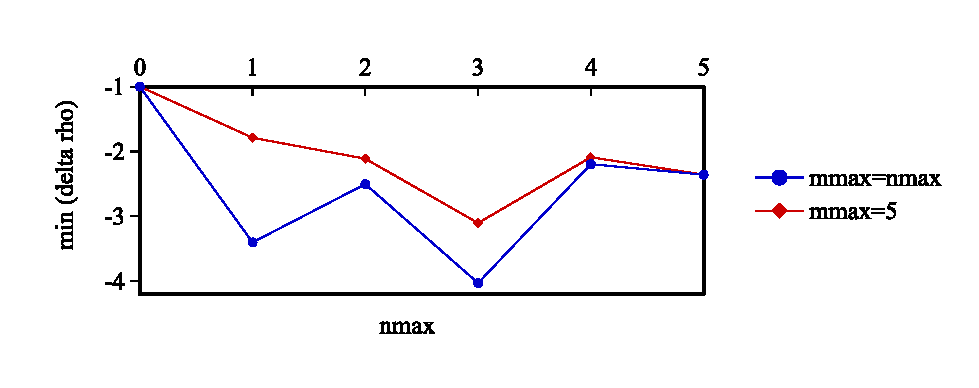
\includegraphics[bb=0bp 10bp 454bp 160bp,width=0.75\columnwidth]{_figure/results/min_delta_rho}
\par\end{centering}
\caption[The minimum value of $\Delta\rho(\mathbf{r},\mathbf{\Omega})/\rho_{0}$
after a forward-backward \acs{GSHT} process]{The minimum value of $\Delta\rho(\mathbf{r},\mathbf{\Omega})/\rho_{0}$
after a forward-backward \acs{GSHT} process with respect to $n_{\max}$.
Computed for a $45^{3}$ grid ($L=25$) for a converged density of
an artificial charged LJ center $\mathrm{CH}_{4}^{+0.4}$. \label{fig:unphysical-rho} }
\end{figure}

Theoretically, we expect this minimum value to approach zero when
increasing $m_{\max}$ or $n_{\max}$. This is not exactly the case.
That means the order of expansion is still far from finding
a tendency. Knowing that $\rho(\mathbf{r},\mathbf{\Omega})/\rho_{0}\rightarrow0$
is at the center of the solute and $\rho(\mathbf{r},\mathbf{\Omega})/\rho_{0}\rightarrow1$
is far from the solute, the error can be termed oblivious within the computing %Oblivious? Is that a scientific term?
capacity ($n_{\max}<5$). That means we cannot rightly expand the
density $\rho$ on \acs{GSH} projections. But this has
much lesser effect on the functional gradient $\gamma$ that we evaluate,
because in a convolution product, $\Delta\hat{\rho}(\mathbf{k},\mathbf{\Omega})$
and the \acs{DCF} $\hat{c}(k,\mathbf{\Omega}_{1},\mathbf{\Omega}_{2})$
can both be expanded, and the product of higher order terms vanishes more %'expended' or 'expanded'? Hmmm....
easily. Later we will show that the profile of $\gamma$ and the
free energy $\mathcal{F}_{\mathrm{exc}}$ can already converge within
$n_{\max}<5$.

\section{Comparison between branches}

As shown in figure \ref{fig:Possible-algorithms}, if we fix $\Delta\rho(\mathbf{r},\mathbf{\Omega})$
to a recombination of \acs{GSH} projections, all methods using the
same \acs{DCF} should give mathematically identical results. The
most direct comparison is the free energy evaluated during one iteration.
To be more strict, it is also worthwhile to compare the profile
of $\gamma$.

\subsection{Difference in energy evaluation}

Illustrated in table \ref{tab:free-energy}, the methods using the same
\acs{DCF} at the same $m_{\max}$, which is mathematically identical
in an infinite condition, give nearly the same results.

\begin{table}[H]
\begin{centering}
\begin{tabular*}{1\linewidth}{@{\extracolsep{\fill}}llll}
\toprule 
\tableheadline{Method} & $n_{\max}$ & \tableheadline{DCF} & \tableheadline{Free Energy} {\footnotesize{}(kJ/mol)}\tabularnewline
\midrule
\texttt{\textbf{\footnotesize{}dipole}} & {\footnotesize{}1} & {\footnotesize{}{[}ref mdft{]}} & {\footnotesize{}13.1915264499904339}\tabularnewline
\texttt{\textbf{\footnotesize{}naive\_dipole}} & {\footnotesize{}1} & {\footnotesize{}{[}ref mdft{]}} & {\footnotesize{}13.1915269013357985}\tabularnewline
\midrule 
\texttt{\textbf{\footnotesize{}naive\_nmax1}} & {\footnotesize{}1} & {\footnotesize{}\citep{puibasset_bridge_2012}{*}} & {\footnotesize{}18.6052247636086854}\tabularnewline
\texttt{\textbf{\footnotesize{}convolution\_standard}} & {\footnotesize{}1} & {\footnotesize{}\citep{puibasset_bridge_2012}{*}} & {\footnotesize{}18.6093390102806886}\tabularnewline
\midrule 
\texttt{\textbf{\footnotesize{}naive\_interpolation}} & {\footnotesize{}2} & {\footnotesize{}\citep{puibasset_bridge_2012}} & {\footnotesize{}26.8444355457069044}\tabularnewline
\texttt{\textbf{\footnotesize{}naive\_standard}} & {\footnotesize{}2} & {\footnotesize{}\citep{puibasset_bridge_2012}} & {\footnotesize{}26.9897310488084479}\tabularnewline
\texttt{\textbf{\footnotesize{}convolution\_standard}} & {\footnotesize{}2} & {\footnotesize{}\citep{puibasset_bridge_2012}} & {\footnotesize{}26.9163932581793155}\tabularnewline
\texttt{\textbf{\footnotesize{}convolution\_asymm}} & {\footnotesize{}2} & {\footnotesize{}\citep{puibasset_bridge_2012}} & {\footnotesize{}26.9163932581793155}\tabularnewline
\texttt{\textbf{\footnotesize{}convolution\_pure\_angular}} & {\footnotesize{}2} & {\footnotesize{}\citep{puibasset_bridge_2012}} & {\footnotesize{}26.9163932581793155}\tabularnewline
\bottomrule
\end{tabular*}
\par\end{centering}
\caption[Free energy calculated during 1 iteration]{Free energy calculated during 1 iteration for a $32^{3}$ grid ($L=20\textrm{Å}$)
for a fake LJ center $\mathrm{CH_{4}^{+0.33}}$, using a converged
density as input. Here $m_{\max}=n_{\max}$. \textcolor{red}{``{*}''
means ancient DCF, not so much difference.}\label{tab:free-energy}}
\end{table}
 

The slight difference between \texttt{\textbf{naive\_nmax1}} and \texttt{\textbf{convolution\_standard}}
at $m_{\max}=1$ is due to the artificial decoration at $k$-border
shown in later sections, and the difference between \texttt{\textbf{naive\_interpolation}}
and \texttt{\textbf{naive\_standard}} and \texttt{\textbf{convolution}}
methods are also acceptable, as it is natural to be slightly different
due to the interpolation error and the \acs{GSH} expansion (the $\rho$
recombination of \acs{GSH} projections will be discussed later).
This supports the theory that we do not need the same order of \acs{GSH}
expansion for $\gamma$ as for $\Delta\rho$.

\subsection{A single k-kernel\label{subsec:A-single-k-kernel}}

Firstly, we are interested in the local paths from $\Delta\hat{\rho}_{\mu'\mu}^{m}(\mathbf{k})$
to $\hat{\gamma}_{\mu'\mu}^{m}(\mathbf{k})$ that can be tested
independently for a certain $\mathbf{k}$. Referring to figure \ref{fig:k-kernel},
four algorithms are available for such a purpose.

\begin{figure}[h]
\begin{centering}
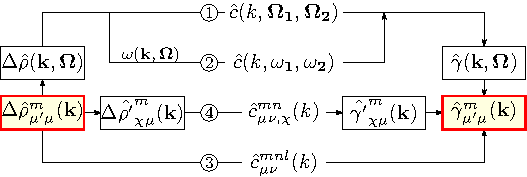
\includegraphics{_figure/algorithms_q}
\par\end{centering}
\caption{Schema of a k-kernel test \label{fig:k-kernel} }
\end{figure}

The program that compares each element of $\hat{\gamma}_{\mu'\mu}^{m}(\mathbf{k})$
issued from these four algorithms for a given $\Delta\hat{\rho}_{\mu'\mu}^{m}(\mathbf{k})$
is done by Mr. Luc Belloni. He shows that the $\hat{\gamma}_{\mu'\mu}^{m}(\mathbf{k})$
for the four algorithms are strictly identical. This means the final
result of energy and structure is independent of the choice of path
inside a $k$-kernel, if $\Delta\hat{\rho}(\mathbf{k},\mathbf{\Omega})$
can be fully expanded on \acs{GSH}s.

\subsection{k-border effect\label{subsec:k-border-effect}}

Here we test the whole process shown in figure \ref{fig:Possible-algorithms},
with $\Delta\rho(\mathbf{r},\mathbf{\Omega})$ generated from a recombination
of \acs{GSH} projections. First off, we compare the three \texttt{\textbf{convolution}}
algorithms passing by \acs{GSH} expansion. For a $64^{3}$ grid,
$n_{\max}=3$, the three algorithms \texttt{\textbf{convolution\_standard}},
\texttt{\textbf{convolution\_asymm}}, and \texttt{\textbf{convolution\_pure\_angular}}
give the same free energy but somewhat different results when comparing
each element of $\gamma(\mathbf{r},\mathbf{\Omega})$. The perceived difference
seems to decrease when we increase the number of grid points. Moreover, the
projections $\gamma_{\mu'\mu}^{m}(\mathbf{r})$ which should be purely
real as explained in $\mathsection$\ref{subsec:Reduction-by-symmetry},
have a slight imaginary part. Surprisingly, for a $65^{3}$ grid,
it gives numerically the same result for all three algorithms
at machine precision.{*} \marginpar{{*} The detailed value of $\gamma$ which the paragraph of description
is based on has not been noted, as it was regarded as a bug in the
code at that time, and the code has since been modified. To redo
such a process takes a lot of time.}

The difference between these methods is found to be a special $k$-border
effect linking to even number grids.

As the symmetry
\begin{equation}
\Delta\hat{\rho'}_{\chi\mu}^{m}(\mathbf{k})=(-)^{m+\mu+\chi}\Delta\hat{\rho'}_{\chi,-\mu}^{m*}(-\mathbf{k})\label{eq:2-1}
\end{equation}
 is generated by two symmetries
\begin{equation}
\Delta\hat{\rho}_{\mu'\mu}^{m}(\mathbf{k})=(-)^{\mu'+\mu}\Delta\hat{\rho}_{-\mu',-\mu}^{m*}(-\mathbf{k})\label{eq:1-1}
\end{equation}
\begin{equation}
R_{\mu'\chi}^{m}(\hat{k})=(-)^{m+\mu'+\chi}R_{-\mu',\chi}^{m}(-\hat{k})\label{eq:3-1}
\end{equation}

For the points ``at border'', it's safe to say that after the FFT where %This sentence makes no sense to me. Not sure if this helped.
the point having $\pm k_{i}=k_{i}^{\mathrm{max}}$, $i=1,2,3$, for
example for $k_{1},$

\[
\Delta\hat{\rho}_{\mu'\mu}^{m}(\pm k_{1},k_{2},k_{3})=\Delta\hat{\rho}_{\mu'\mu}^{m}(k_{1}^{\mathrm{max}},k_{2},k_{3})
\]
is naturally put in the same array by FFT for the grids of an even
number,\marginpar{For example, for a grid 1D, the FFT having 6 points gives the values
for indices 0,1,2,3,-2,-1, and the FFT having 7 points gives the values
for 0,1,2,3,-3,-2,-1.} as shown in figure \ref{fig:k-border-effect}. 

\begin{figure}[h]
\begin{centering}
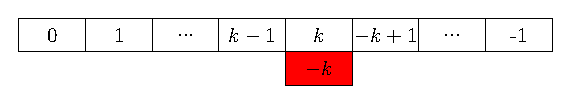
\includegraphics{_figure/k-border}
\par\end{centering}
\caption{$k$-border effect\label{fig:k-border-effect}}
\end{figure}

As \acs{FFT} possesses periodicity, the symmetry \ref{eq:1-1} can
always be respected at the border. However, as
\begin{equation}
R_{-\mu',\chi}^{m}(-\hat{k}\equiv(-k_{1},-k_{2},-k_{3}))\neq R_{\mu',\chi}^{m}(k_{1}^{\mathrm{max}},-k_{2},-k_{3})
\end{equation}
the symmetries (\ref{eq:3-1}) and (\ref{eq:2-1}) are not respected
for these points. In the backward process, if we make sense of all
the $\gamma_{\mu'\mu}^{m}(\mathbf{k})$, as
\[
\gamma_{\mu'\mu}^{m}(-\hat{k}\equiv(-k_{1},-k_{2},-k_{3}))\neq\gamma_{\mu'\mu}^{m}(k_{1}^{\mathrm{max}},-k_{2},-k_{3})
\]
the symmetry
\begin{equation}
\gamma_{\mu'\mu}^{m}(\mathbf{k})=(-)^{\mu'+\mu}\gamma_{-\mu',-\mu}^{m*}(-\mathbf{k})\label{eq:1-1}
\end{equation}
is not respected totally, and this imposes that $\gamma_{\mu'\mu}^{m}(\mathbf{r})$
has an imaginary part. This imaginary part has been omitted implicitly
in the ``real to complex'' \acs{FFT} process used in, for example,
\texttt{\textbf{convolution\_standard}}, for \acs{FGSHT}, or \texttt{\textbf{convolution\_pure\_angular}}
for FFT3D process. That is to say, we keep only the part of nonnegative
$\mathbf{k}$ or nonnegative $\mu$, supposing that the part we
omit respects the symmetry.

The correct way to treat this issue is to artificially impose at the
border:
\begin{equation}
R_{\mu',\chi}^{m}(k_{i}^{\mathrm{max}})=\frac{1}{2}\left[R_{\mu',\chi}^{m}(k_{i})+R_{\mu',\chi}^{m}(-k_{i})\right]
\end{equation}
where $i$ is the conflict index in figure \ref{fig:k-border-effect}.
If more than one dimension is in conflict, this process can be done
twice (4 terms for ``edges'' of the cube) or three times (8 terms
for ``vertices''). The point $\mathbf{k}=\hat{0}$ is different;
as it was defined along $z$ axes to avoid implementation crash, it
doesn't respect eq. (\ref{eq:3-1}) or (\ref{eq:2-1}). But
this is negligible when compared to hundreds of thousands of total points.

The energies given by \texttt{\textbf{naive\_standard}} and the \texttt{\textbf{convolution}}
algorithms are identical for a $65^{3}$ and $n_{\max}=3$ grid, but
the element of $\gamma(\mathbf{r},\mathbf{\Omega})$ has a mysterious
difference at order of $10^{-2}$ which seems to be aleatory. A test redone %Nice word, 'aleatory', but is it appropriate for a scientific work?
for a $45^{3}$ grid is shown in figure \ref{fig:Difference-in-gamma}.

\begin{figure}[H]
\begin{centering}
\subfloat[$\delta\hat{\gamma}(\mathbf{k},\mathbf{\Omega})$]{\begin{centering}
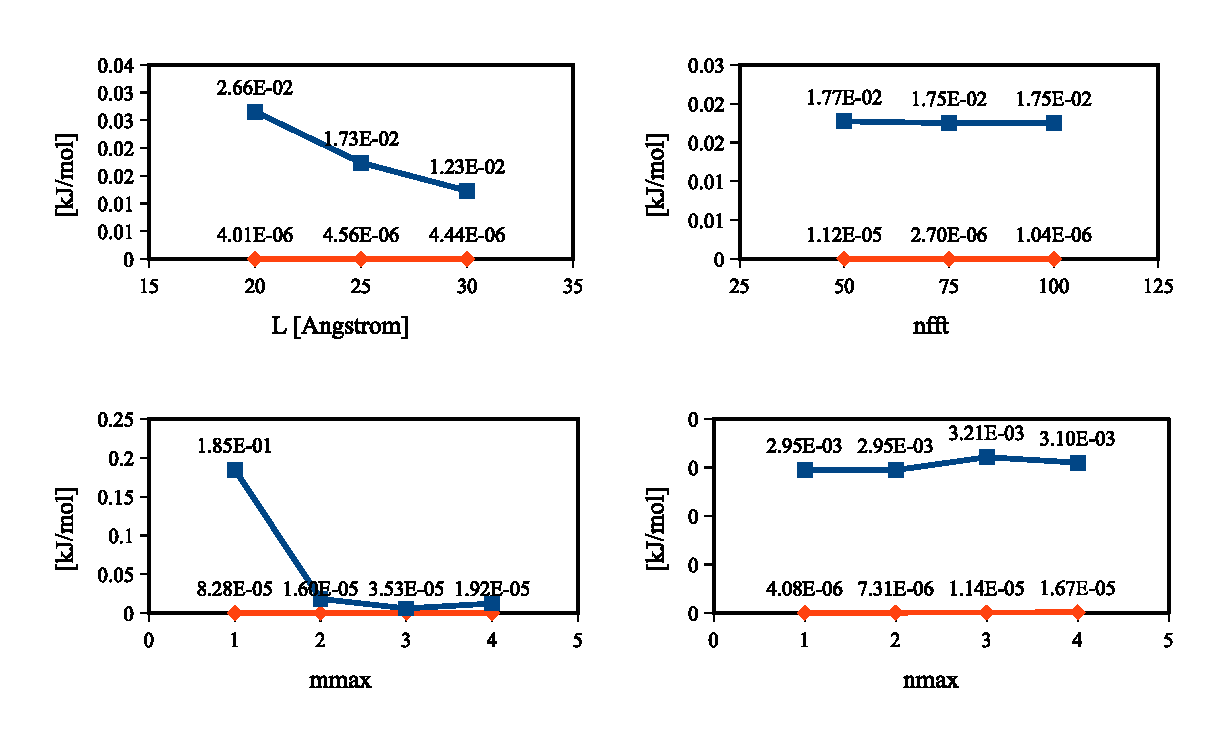
\includegraphics[width=0.75\columnwidth]{_figure/results/diff_k_gamma}
\par\end{centering}

}
\par\end{centering}
\begin{centering}
\subfloat[$\delta\gamma(\mathbf{r},\mathbf{\Omega})$]{\begin{centering}
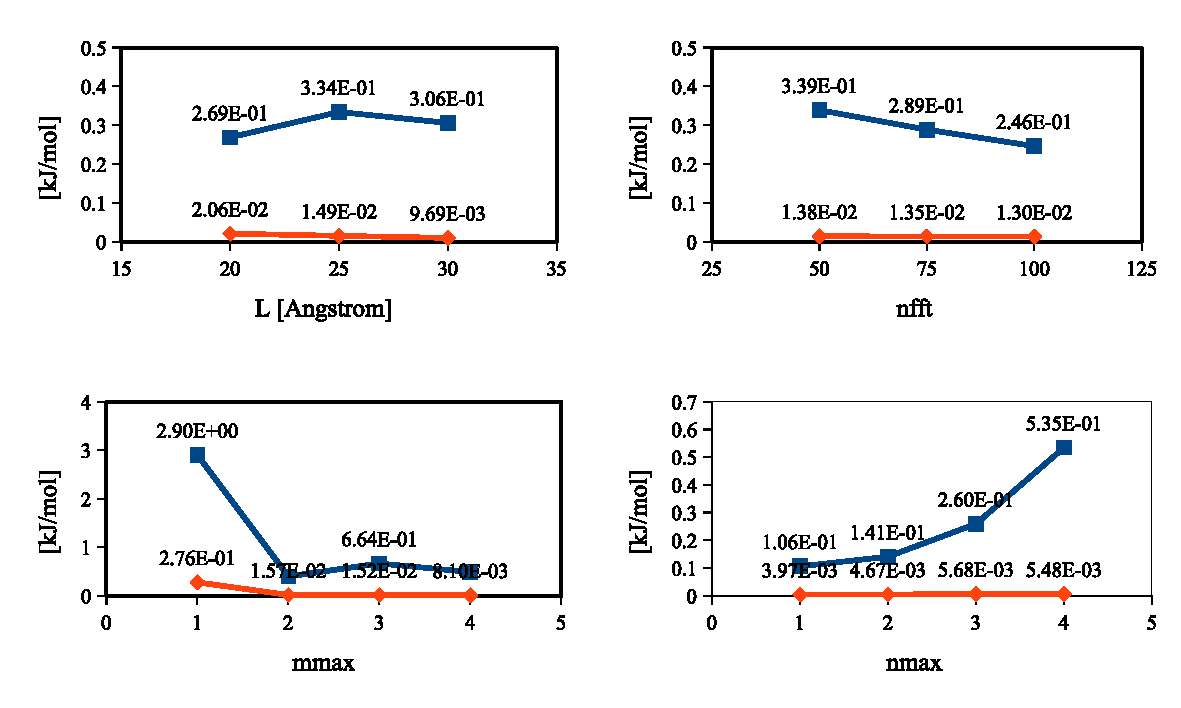
\includegraphics[width=0.75\columnwidth]{_figure/results/diff_gamma}
\par\end{centering}
}
\par\end{centering}
\caption[Maximum and average difference in $\hat{\gamma}(\mathbf{k},\mathbf{\Omega})$
and $\gamma(\mathbf{r},\mathbf{\Omega})$]{Maximum and average difference in $\hat{\gamma}(\mathbf{k},\mathbf{\Omega})$
and $\gamma(\mathbf{r},\mathbf{\Omega})$, for tests of different
box length$L$, different number of grid nfft in one dimension, $n_{\max}=1,4$
for $m_{\max}=n_{\max}$, and $n_{\max}=1,4$ for $m_{\max}=5$.\label{fig:Difference-in-gamma}}
\end{figure}

We can conclude very rudely that this error depends on the angular
quadrature $m_{\max}$. The dependence is natural, as the difference
between algorithms \texttt{\textbf{naive}} and \texttt{\textbf{convolution}}
is the treatment of the angular part. There is also a dependence on
$L$ in the $k$-space, but after \acs{FFT} it is mixed. The augmentation
of error in the $n_{\max}$ chart is unnatural, implying there is
perhaps a still bug in the code.

In a word, this mysterious difference cannot be yet explained, as
the \texttt{\textbf{naive}} methods does not have the $k$-border
effect linked to symmetry, on the other hand we used a odd grid, we
could not yet distinguish that it is a bug in the implementation,
in the test or in the theory. The projections $\gamma_{\mu\nu}^{mnl}(r)$
of this two algorithms seems to be identical (figure \ref{fig:gamma-proj}),
it is to say, the global structure of this two algorithms are almost
the same, and the error would not be very decisive.

\begin{figure}[h]
\begin{centering}
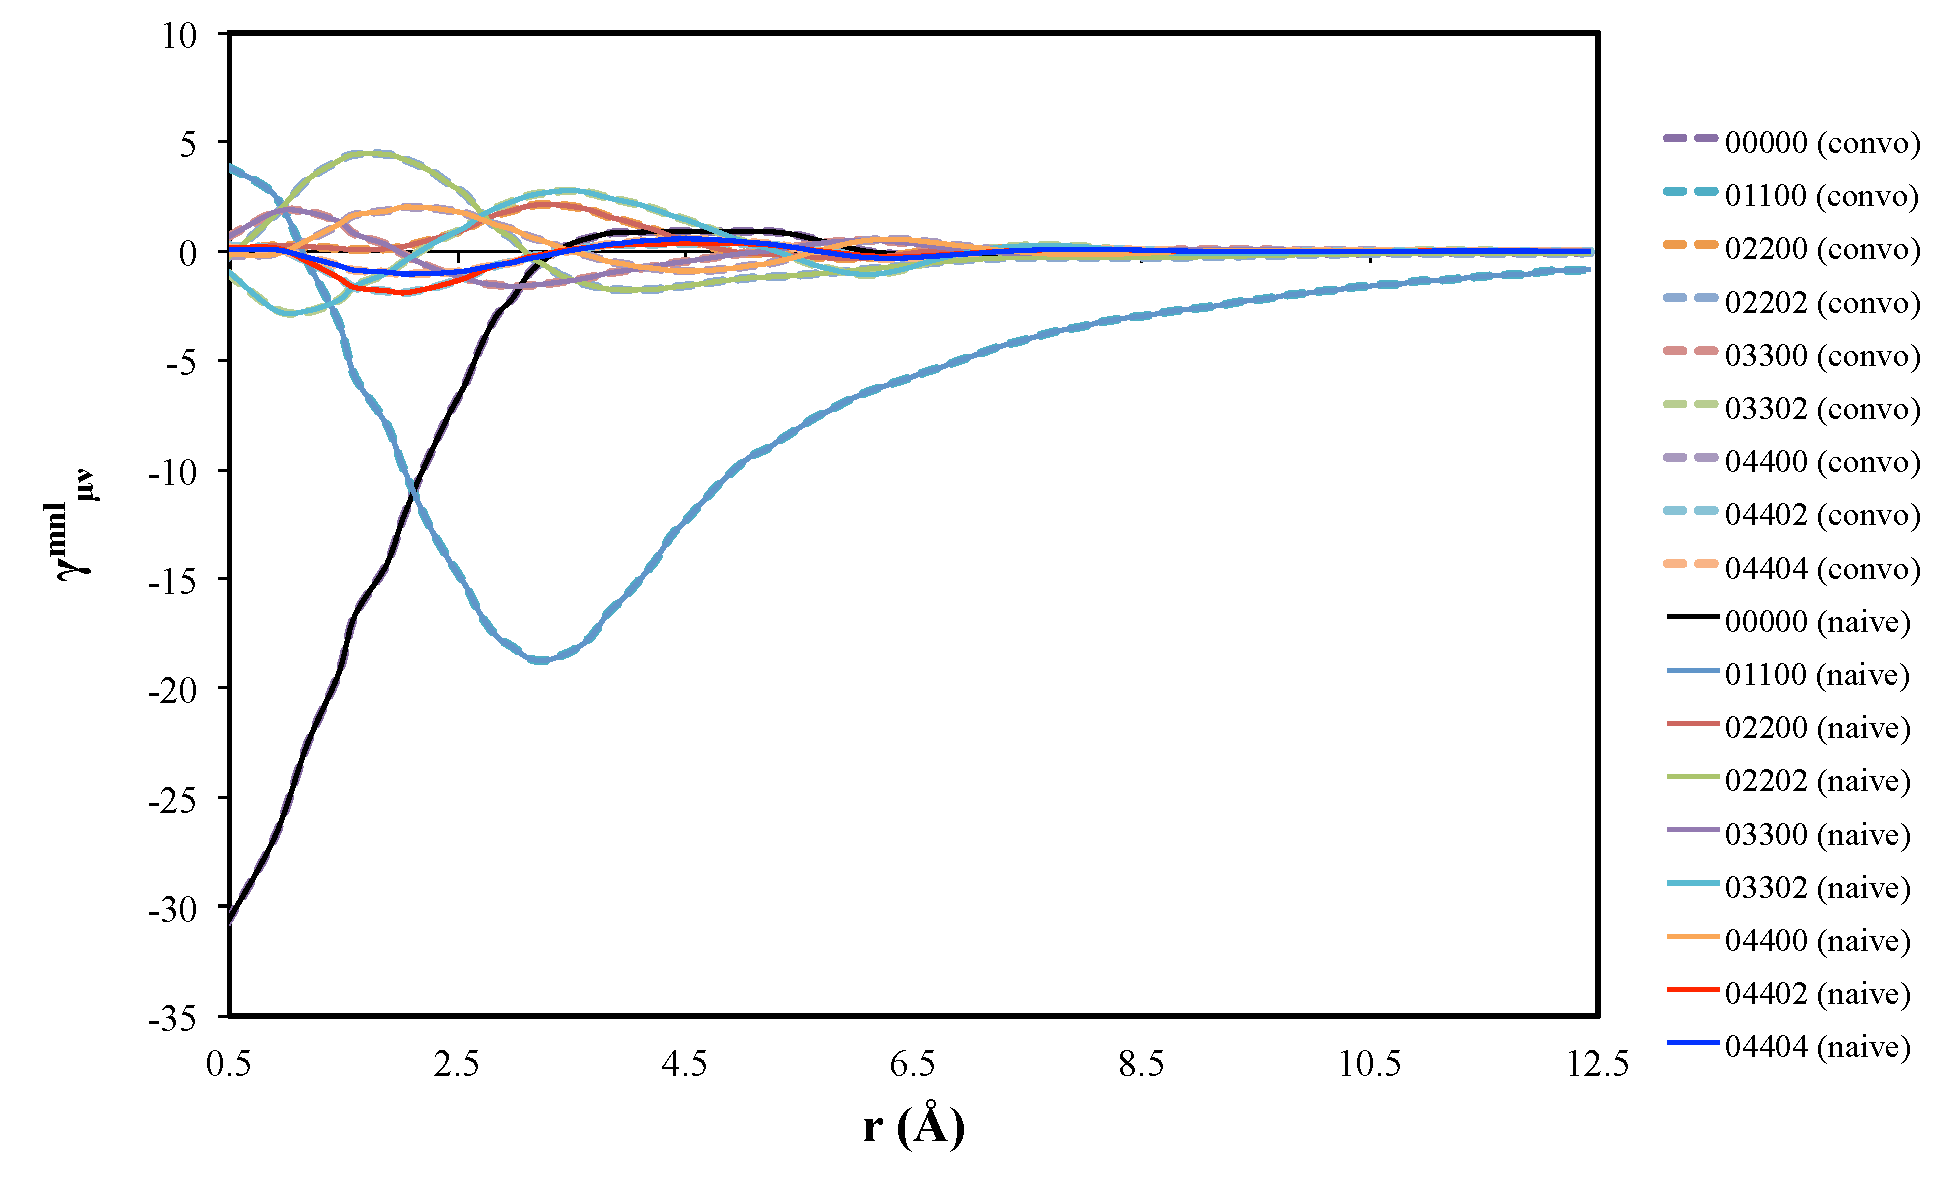
\includegraphics[width=0.65\columnwidth]{_figure/results/gamma_proj}
\par\end{centering}
\caption{A selection of rotational invariant projections $\gamma_{\mu\nu}^{mnl}(r)$
for a $65^{3}$ grid\label{fig:gamma-proj}}
\end{figure}


\section{Intrinsic variation of free energy\label{sec:Intrinsic-variation-of}}

Before study of free energy dependence on angular algorithms, we are
interested in the grid dependance, with can have an influence to the
tests later.

\begin{figure}[H]
\begin{centering}
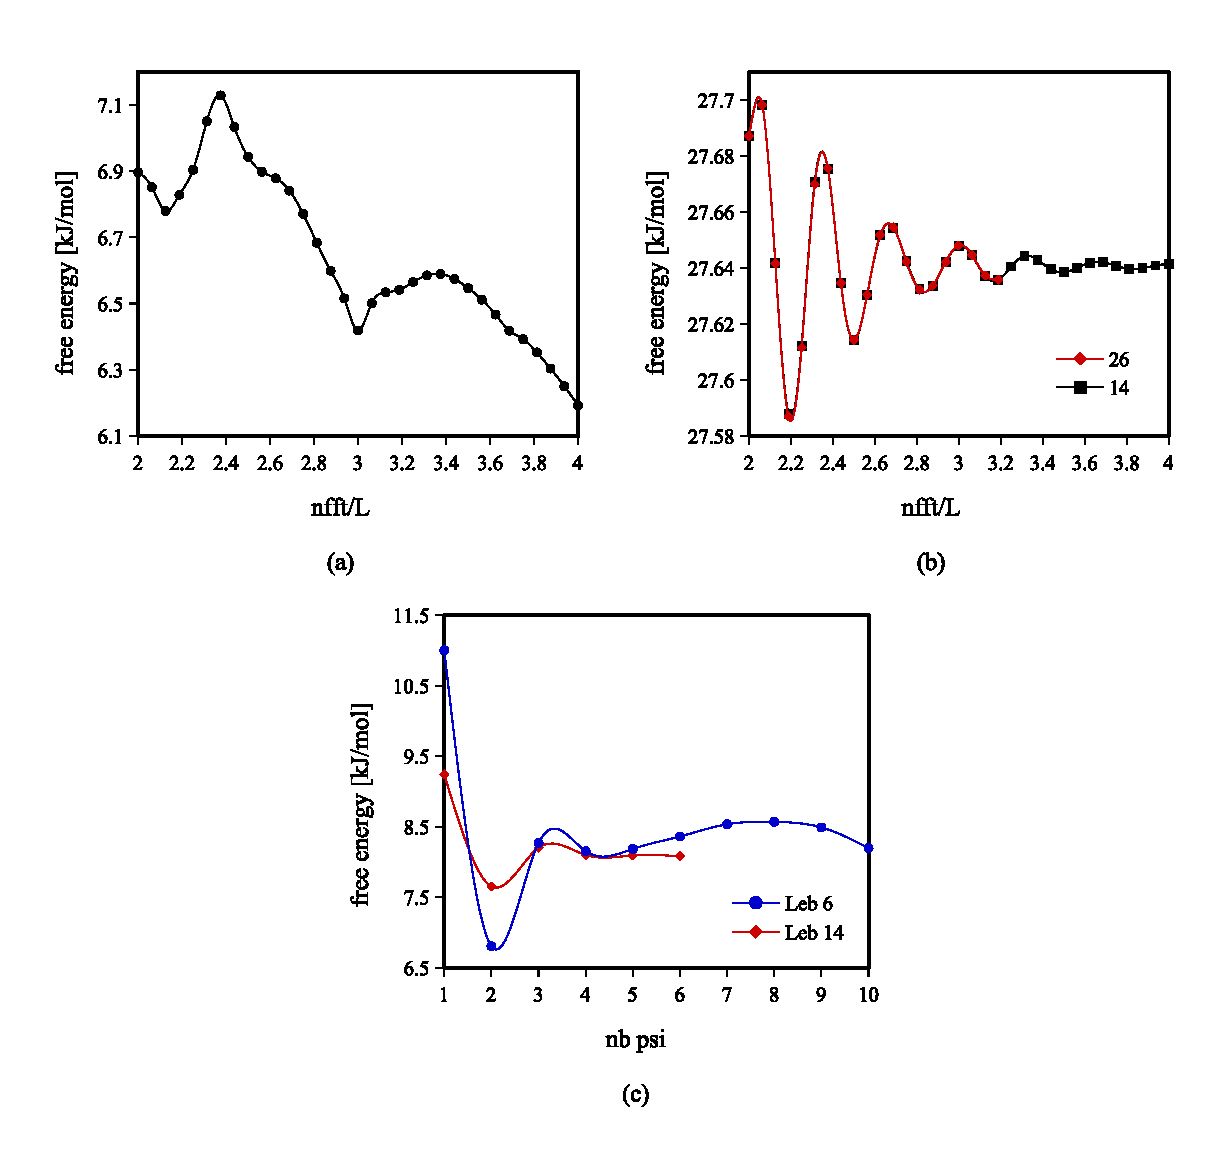
\includegraphics[bb=0bp 20bp 567bp 519bp,width=0.75\columnwidth]{_figure/results/grid_reso}
\par\end{centering}
\caption[Space-grid and $\Psi$ dependence of code MDFT]{Space-grid and $\Psi$ dependence of code MDFT. $L=32$. (a) $\mathrm{CH_{4}^{+0.33}}$
using dipole DCF with $m_{\max}=1$; (b) $\mathrm{CH_{4}}$ using
DCF of $m_{\max}=5$, Lebedev quadrature of order 1 and 2; (c) acetone
using dipole DCF and Lebedev quadrature, varying $\Psi$, nfft=128.
\label{fig:Space-grid-and-psi-dependence}}
\end{figure}

As shown in figure \ref{fig:Space-grid-and-psi-dependence} (a) and
(b), there is a dependence of calculated free energy on the space
grid resolution. for a charged solute, the energy has tendency to
decrease when increasing the resolution of grid (nfft). And this decrease
does not link to the border correction mentioned in $\mathsection$\ref{chpt:thermodynamic-quantities},
as the box length and the charge remain the same for the whole set
of test. From (b) we consider that at least 3 points grid in one dimension
per Angstrom is needed to reduce the uncertainty due to grid resolution.
Figure (c) fixed the Lebedev quadrature for $\Theta$ and $\Phi$,
but leaved varying the $\Psi$. We can also see a dependence on $\Psi$.
which does not vanish when increasing the resolution of grid. As during
the whole thesis the $\Psi$ is theoretically fixed in the same order
with $\Theta$ and $\Phi$, this remains an issue for further verification.
We can roughly conclude that an error around 1 kJ/mol is common for
this code.

\section{Series of charged LJ centre}

To valid the method, we chose a series of LJ centre, which possess
the LJ parameters of $\mathrm{C}\mathrm{H}_{4}$ in \textcolor{red}{{[}ref{]}},
and have a various charge from -1.0 to 1.0 (table \ref{tab:Parameters-of-charged-met}).\marginpar{For both IET, and DM results, 298K is used according to habitude instead
of 303K recommended in reference \citep{SPC/E}. For MDFT, 300K and
298K are used.}

\begin{table}[h]
\begin{centering}
\begin{tabular*}{1\linewidth}{@{\extracolsep{\fill}}lllllll}
\toprule 
\tableheadline{Charge} & $\sigma$ {[}$\textrm{Å}${]} & $\epsilon$ {[}$\mathrm{kJ\cdot mol^{-1}}${]} & $x$ {[}$\textrm{\AA}${]} & $y$  {[}$\textrm{\AA}${]} & $z$ {[}$\textrm{\AA}${]} & \tableheadline{Number Density} {[}$\lyxmathsym{\AA}^{-3}${]}\tabularnewline
\midrule
-1.0 to 1.0 & 3.73  & 1.23  & 0 & 0 & 0 & 0.0332891 \textcolor{red}{{[}ref,temperature{]}}\tabularnewline
\bottomrule
\end{tabular*}
\par\end{centering}
\caption{Parameters of charged Lenard-Jones centre (modified from $\mathrm{C}\mathrm{H}_{4}$)
\label{tab:Parameters-of-charged-met}}
\end{table}


\subsection{Box length dependance and charge dependance of free energy}

As discussed in section \ref{chpt:thermodynamic-quantities}, for
single ions, two types of corrections need to be added on the free
energy, which depend on the box length and and charge of the ion.
To verify these dependence, we implement a systematic calculation
from charge, using 3 different methods, where the parameters are shown
in table \ref{tab:parameters-ch4}. It should be noted that, the \texttt{\textbf{naive\_interpolation}}
only used 14 Lebedev and 3 $\Psi$ angles to converge, which gives
exactly the same result with 26 Lebedev and 4 $\Psi$ angles, that
means, the \texttt{\textbf{naive}} methods do not need an order of
quadrature $m_{\max}$ to be greater than the order of DCF $n_{\max}$.
The -1 side has problem of convergence, and all the converged results
are presented.

\begin{table}[h]
\begin{centering}
\begin{tabular*}{1\linewidth}{@{\extracolsep{\fill}}llll}
\toprule 
\tableheadline{Method} & nfft/$L$ & $m_{\max}$ & $n_{\max}$\tabularnewline
\midrule
\texttt{\textbf{naive\_nmax1}} & 3 & 1 & 1\tabularnewline
\texttt{\textbf{naive\_interpolation}} & 3 & 2 (Leb) & 5\tabularnewline
\texttt{\textbf{convolution\_standard}} & 3 & 1 & 1\tabularnewline
\bottomrule
\end{tabular*}
\par\end{centering}
\caption{Methods and parameters for $\mathrm{C}\mathrm{H}_{4}$ series test.
{*} Leb is Lebedev quadrature, with is mathematically equivalent with
Gauss-Legendre quadrature but only ˜2/3 angles.\label{tab:parameters-ch4}}
\end{table}

The direct results collection are shown in figure \ref{fig:ch4_nmax1_lmn},
\ref{fig:ch4_nmax5_inter} and \ref{fig:ch4_nmax1_new} at the end
of this section. We can see that the dependence of box length for
each charge is almost linear, except the charge between $\left[-0.2,0.2\right]$.
This means, the influence of box length is much greater than the intrinsic
variation of result that mentioned in \ref{sec:Intrinsic-variation-of}.
The charge dependency is traced in figure \ref{fig:Quadratic-charge-dependence},
using all the number of slopes with respect to the square of their
charge ($q^{2}$). A linear regression is done to give the slope 1937.8
$\mathrm{kJ}\cdot\mathrm{mol^{-1}}\cdot\textrm{Å}$. This slope correspond
to the correction of type-B (normalized to give the right unity):
\begin{equation}
\dfrac{\xi}{2}\left(1-\dfrac{1}{\varepsilon}\right)=1943.2\,\mathrm{kJ}\cdot\mathrm{mol^{-1}}\cdot\textrm{Å}
\end{equation}

\begin{figure}[H]
\begin{centering}
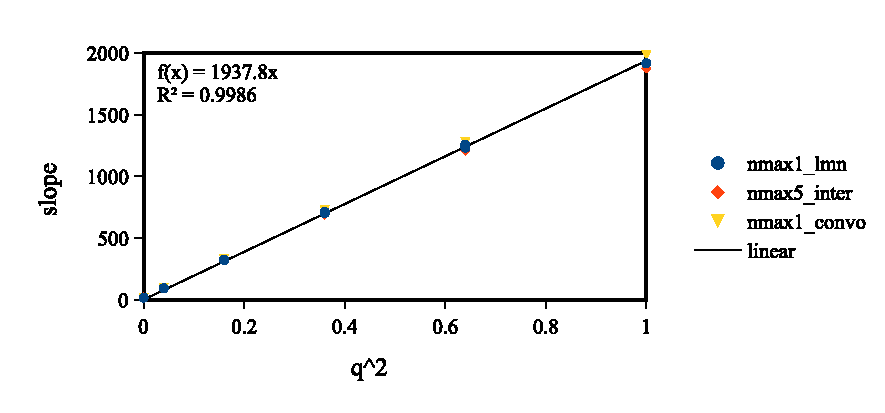
\includegraphics[bb=0bp 20bp 425bp 178bp,scale=0.6]{_figure/results/ch4_slope}
\par\end{centering}
\caption{Quadratic charge dependence of free energy of $\mathrm{C}\mathrm{H}_{4}$
centre series\label{fig:Quadratic-charge-dependence}}
\end{figure}
The intercept values in each of figure \ref{fig:ch4_nmax1_lmn} to
\ref{fig:ch4_nmax1_new} correspond to the free energy of an infinite
box. The \acs{IET} results are done with $R_{\max}=102.4\textrm{Å}$,
and need a correction of $-2.556k_{\mathrm{B}}T$. \textcolor{red}{(need
more details.)} The differences in free energy between MDFT and IET
are given in figure \ref{fig:Comparison-to-IET,without-correction}.
The linear regression is done with all existing points in this figure.
The slope 87.653 $\mathrm{kJ}\cdot\mathrm{mol^{-1}}$ corresponds
to the correction of type-C (normalized to give the right unity):
\begin{equation}
\eta\gamma=82.104\mathrm{kJ}\cdot\mathrm{mol^{-1}}\label{eq:eta-gamma}
\end{equation}
These two numbers are a little different, principally due to a lack
of point at the -1 side.

\begin{figure}[h]
\begin{centering}
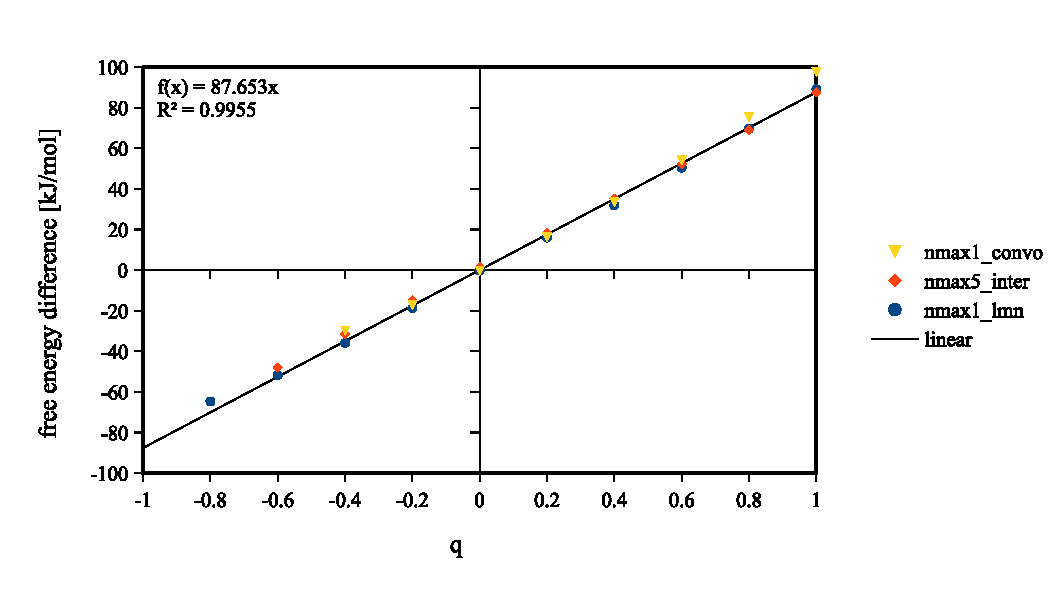
\includegraphics[bb=0bp 20bp 510bp 263bp,scale=0.6]{_figure/results/ch4_diff_energy}
\par\end{centering}
\caption{Comparison to IET, without P-scheme correction\label{fig:Comparison-to-IET,without-correction}}
\end{figure}


\subsection{Comparison with IET after corrections}

The figure \ref{fig:Comparison-to-IET,without-correction} after correction
with eq. (\ref{eq:eta-gamma}) gives figure \ref{fig:Comparison-to-IET,with-corr}.
It is shown that they are not perfectly agreed with each other. The
$n_{\max}=1$ methods have large difference when the charge increased,
especially the \texttt{\textbf{convolution\_standard}} using GSH expansion.
Knowing that during 1 iteration, the \texttt{\textbf{naive\_nmax1}}
and the \texttt{\textbf{convolution\_standard}} only give a slight
difference in free energy (table \ref{tab:free-energy}). The $n_{\max}=5$
have an energy shift about 2 $\mathrm{kJ}\cdot\mathrm{mol^{-1}}$,
which cannot have an explanation. but overall, to have 2 $\mathrm{kJ}\cdot\mathrm{mol^{-1}}$
per 100 $\mathrm{kJ}\cdot\mathrm{mol^{-1}}$ is already a good result.

\begin{figure}[H]
\begin{centering}
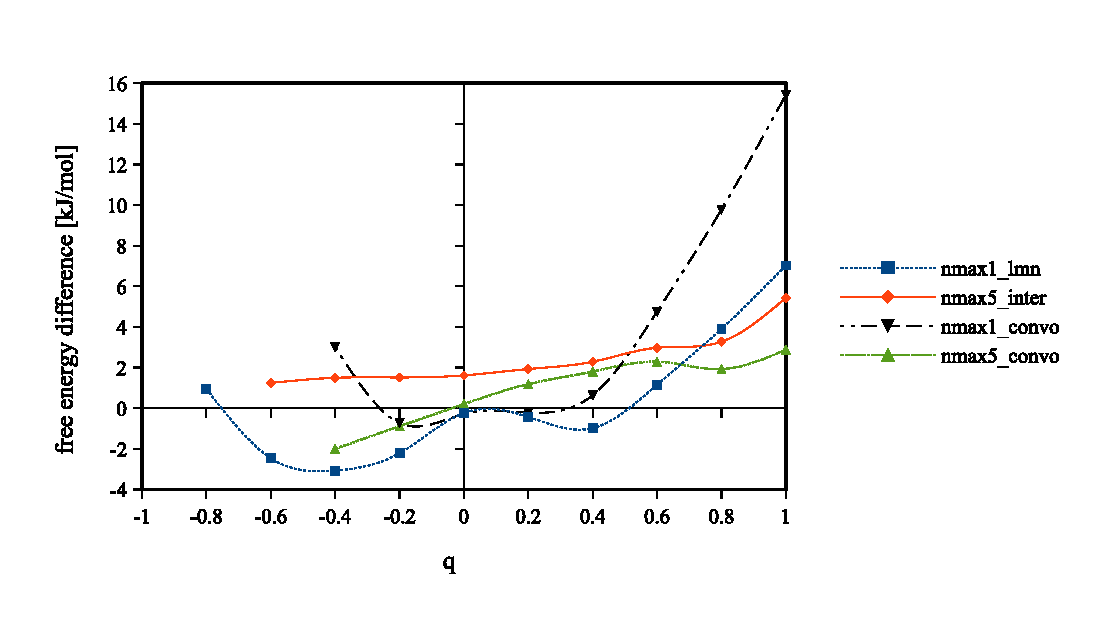
\includegraphics[bb=0bp 20bp 510bp 263bp,scale=0.6]{_figure/results/ch4_diff_inter}
\par\end{centering}
\caption{Comparison to IET, with P-scheme correction\label{fig:Comparison-to-IET,with-corr}}
\end{figure}

The case of $m_{\max}=5$ , $n_{\max}=0,\ldots,5$ with \texttt{\textbf{convolution\_standard}}
is shown in figure \ref{fig:Comparison-to-IET,nmax0-5}. It is interesting
to see how energy evaluate with $n_{\max}$ while fixing $m_{\max}$.
As we said, $\gamma$ is more smooth than $\rho$, that means we can
have $n_{\max}<m_{\max}$ to economize computing cost. Results shows
that within $n_{\max}\geq3$ for $n_{\max}=5$, the error is acceptable.
But again, the dependence on $q$ after correction is in incomprehensible.
And compared to \texttt{\textbf{naive\_interpolation}} in figure \ref{fig:Comparison-to-IET,with-corr},
we see that these error for $n_{\max}=5$ is different.

\begin{figure}[H]
\begin{centering}
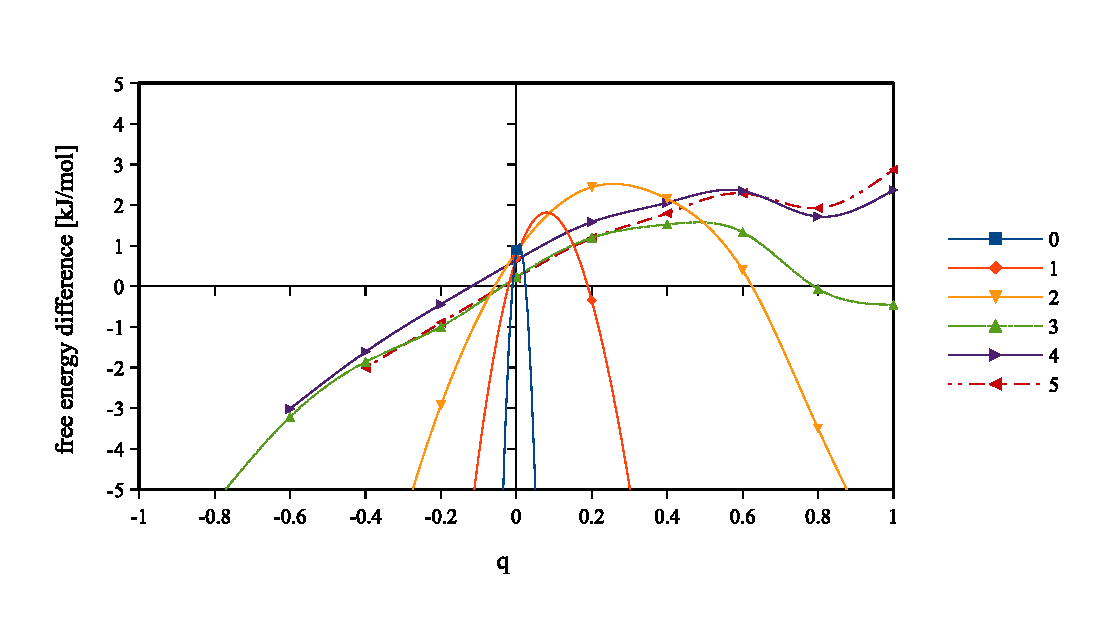
\includegraphics[bb=0bp 20bp 510bp 263bp,scale=0.6]{_figure/results/ch4_diff_mmax5}
\par\end{centering}
\caption{Comparison to IET, with P-scheme correction, $m_{\max}=5$ , $n_{\max}=0,\ldots,5$
\label{fig:Comparison-to-IET,nmax0-5}}
\end{figure}

The profile of $\rho$ can expended on rotational invariants which
is discussed in $\mathsection$\ref{chpt:solvation-structure}. The
comparison with IET is done for three charges, 0, -0.6 and +1. Shown
in figure \ref{fig:Comparison-to-IET.rot_invar}. Watch that the 0
and -1 one of $m_{\max}=5$ corresponds well the result of IEM, but
the -0.6 one have a lot of noise. (In fact, this configuration had
difficulty to converge, and the given energy is not good, thus it
is deleted in figure \ref{fig:Comparison-to-IET,nmax0-5}.) The the
profiles of go much better $m_{\max}=2,3$. Normally, more points
means more precision. It may means that with $m_{\max}=5$ , there
is perhaps a bug of integer overflow that prevent the convergence
for high charges.

\begin{figure}[H]
\begin{centering}
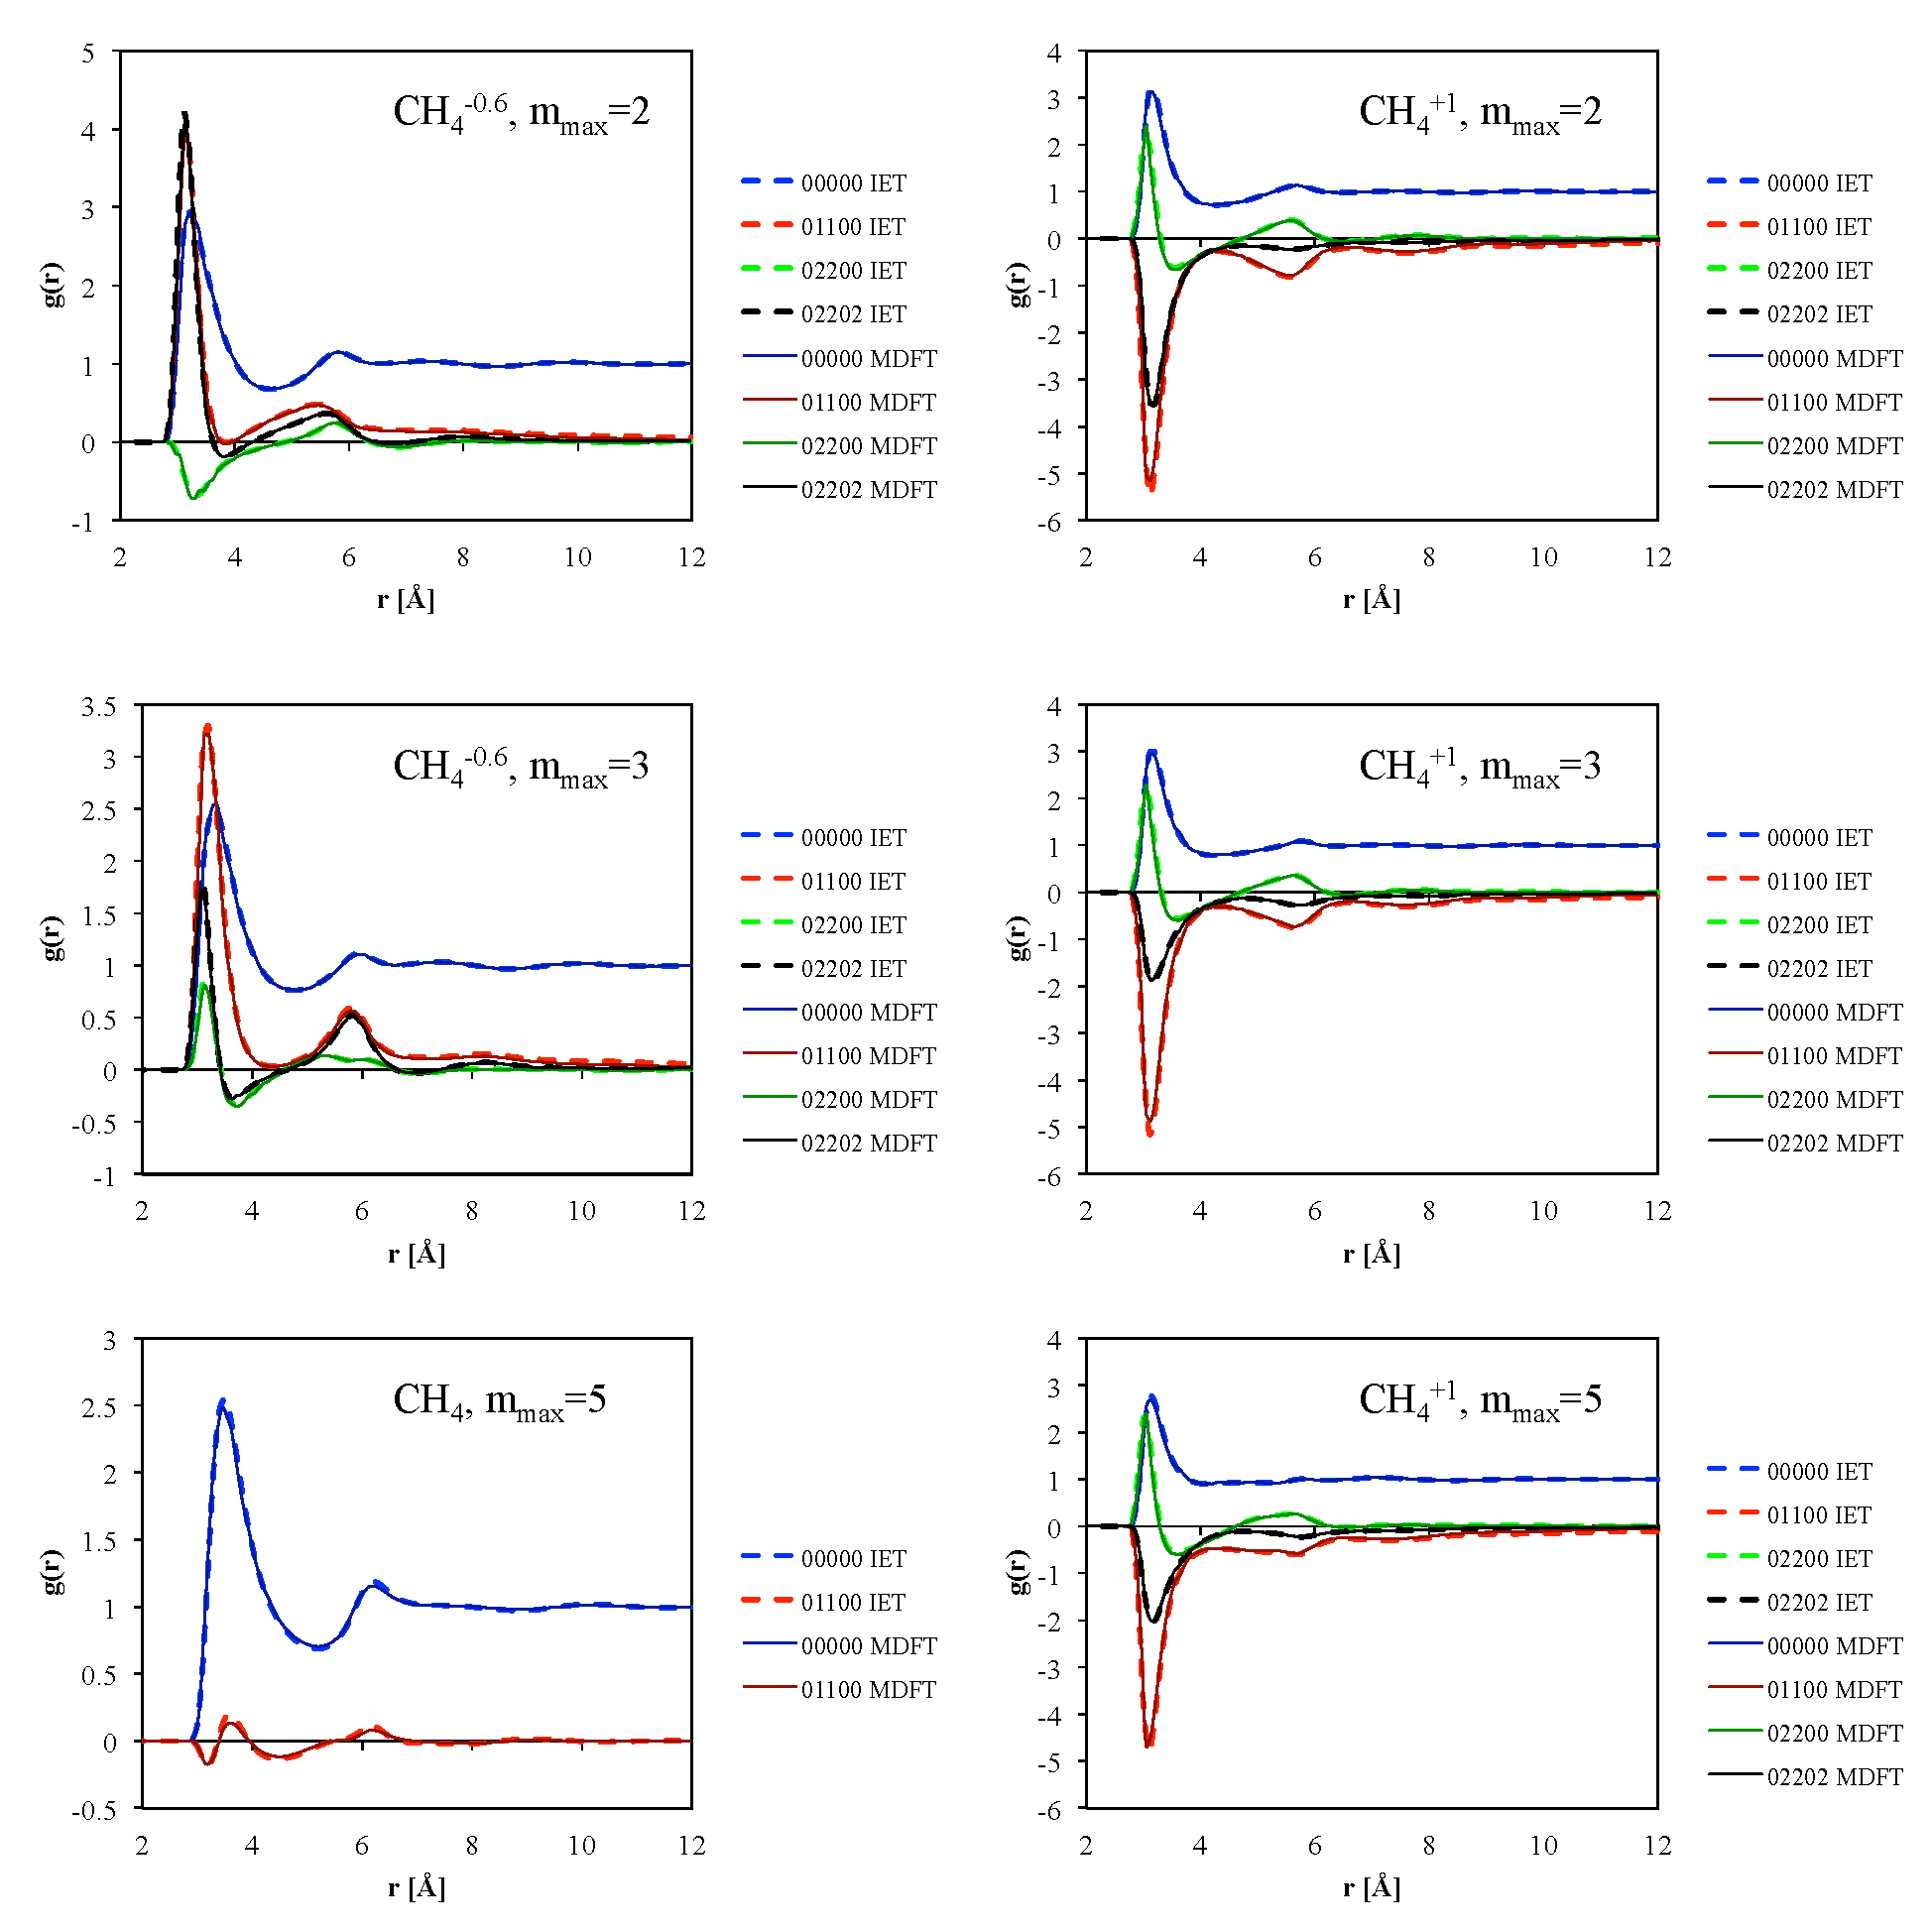
\includegraphics[width=1\columnwidth]{/Users/Hostiphre/Desktop/_M1102/_figure/results/ch4_iet_struct}
\par\end{centering}
\caption{Comparison to IET. Profile of $\rho$ in rotational invariant projections,
L=24, nfft=72.\label{fig:Comparison-to-IET.rot_invar}}
\end{figure}


\subsection{Comparison with MD}

The comparison of RDF with MD results are shown in figure \ref{fig:Comparison-to-MD}.
We can see that for negative charges, there are a lot of shifts.

Discussion...

\begin{figure}[H]
\begin{centering}
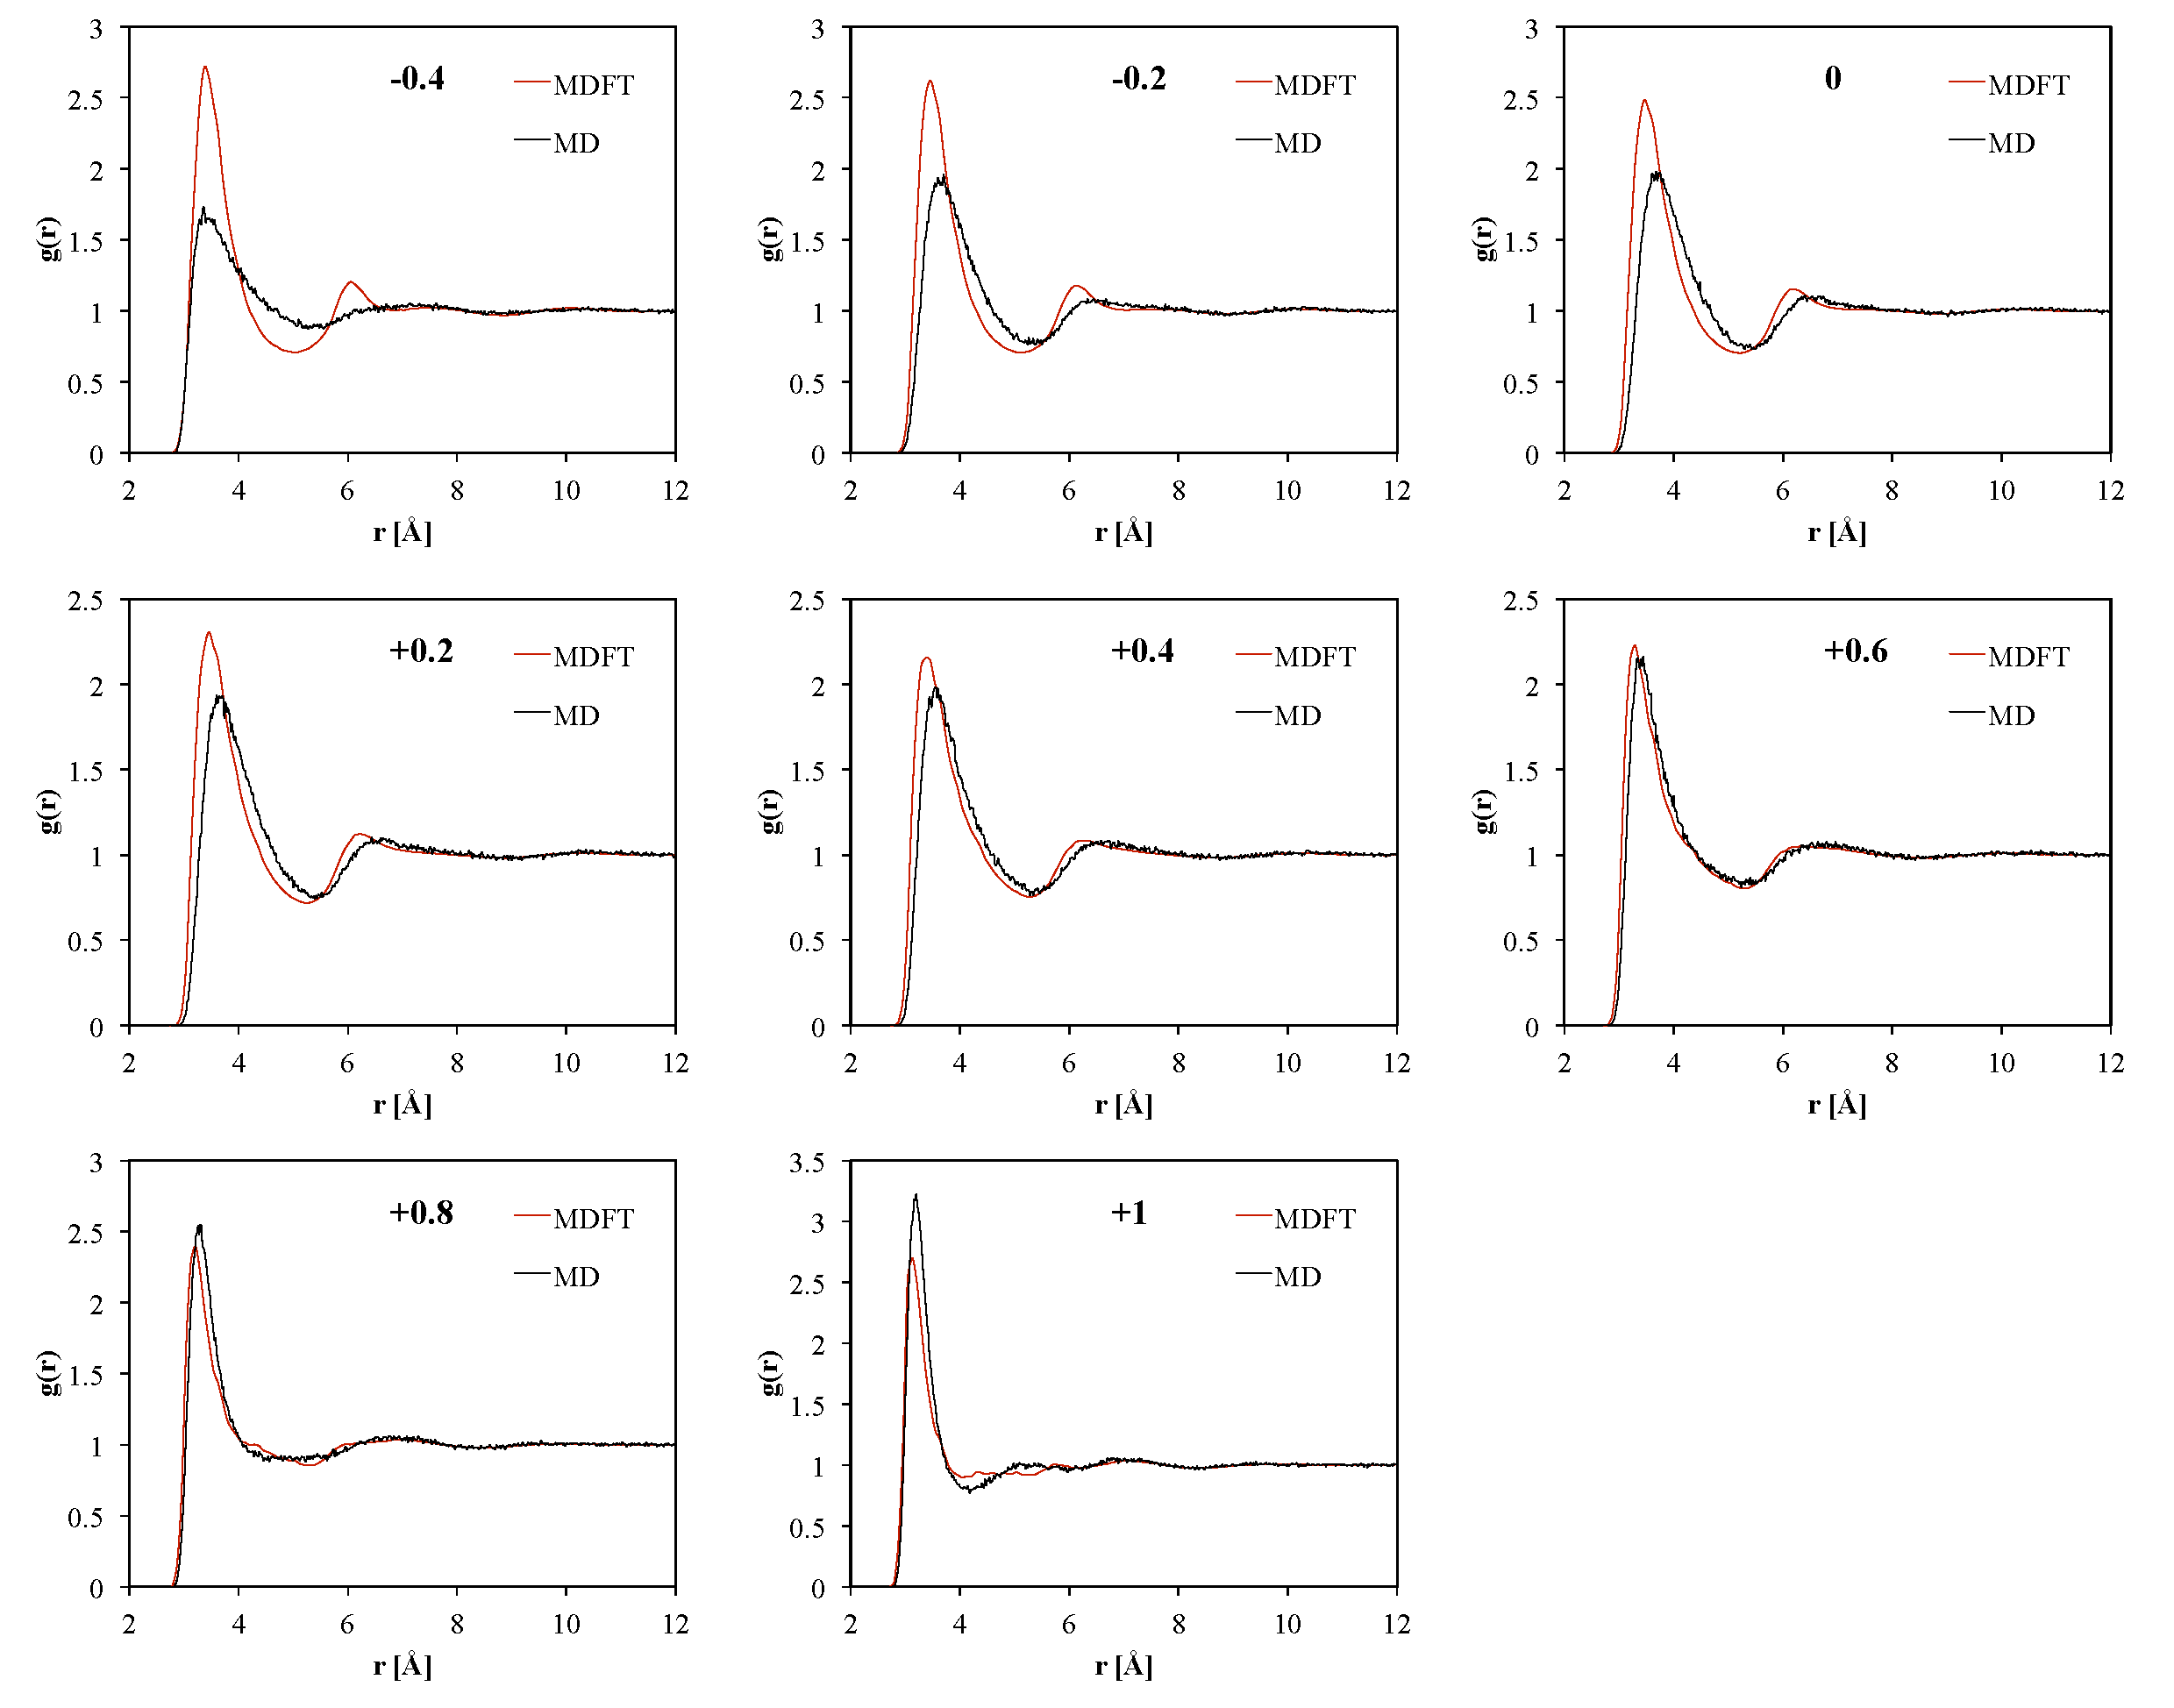
\includegraphics[width=1\columnwidth]{/Users/Hostiphre/Desktop/_M1102/_figure/results/ch4_md}
\par\end{centering}
\caption{Comparison to IET. Profile of $\rho$ in rotational invariant projections.\label{fig:Comparison-to-MD}}
\end{figure}


\section{Premier conclusion}

From the results, we see that MDFT ... ``capable'' to produce the
same result with IEM for single ions. (but have more ability to calculate
3D molecules which is not suitable for spherical coordinates...)

\texttt{\textbf{naive\_interpolation}} is more stable compared to
\texttt{\textbf{convolution}} methods and can use less angles for
convergence, although in the computing time it cannot compare with
\texttt{\textbf{convolution}} methods, which will be discussed later.

\begin{figure}[h]
\begin{centering}
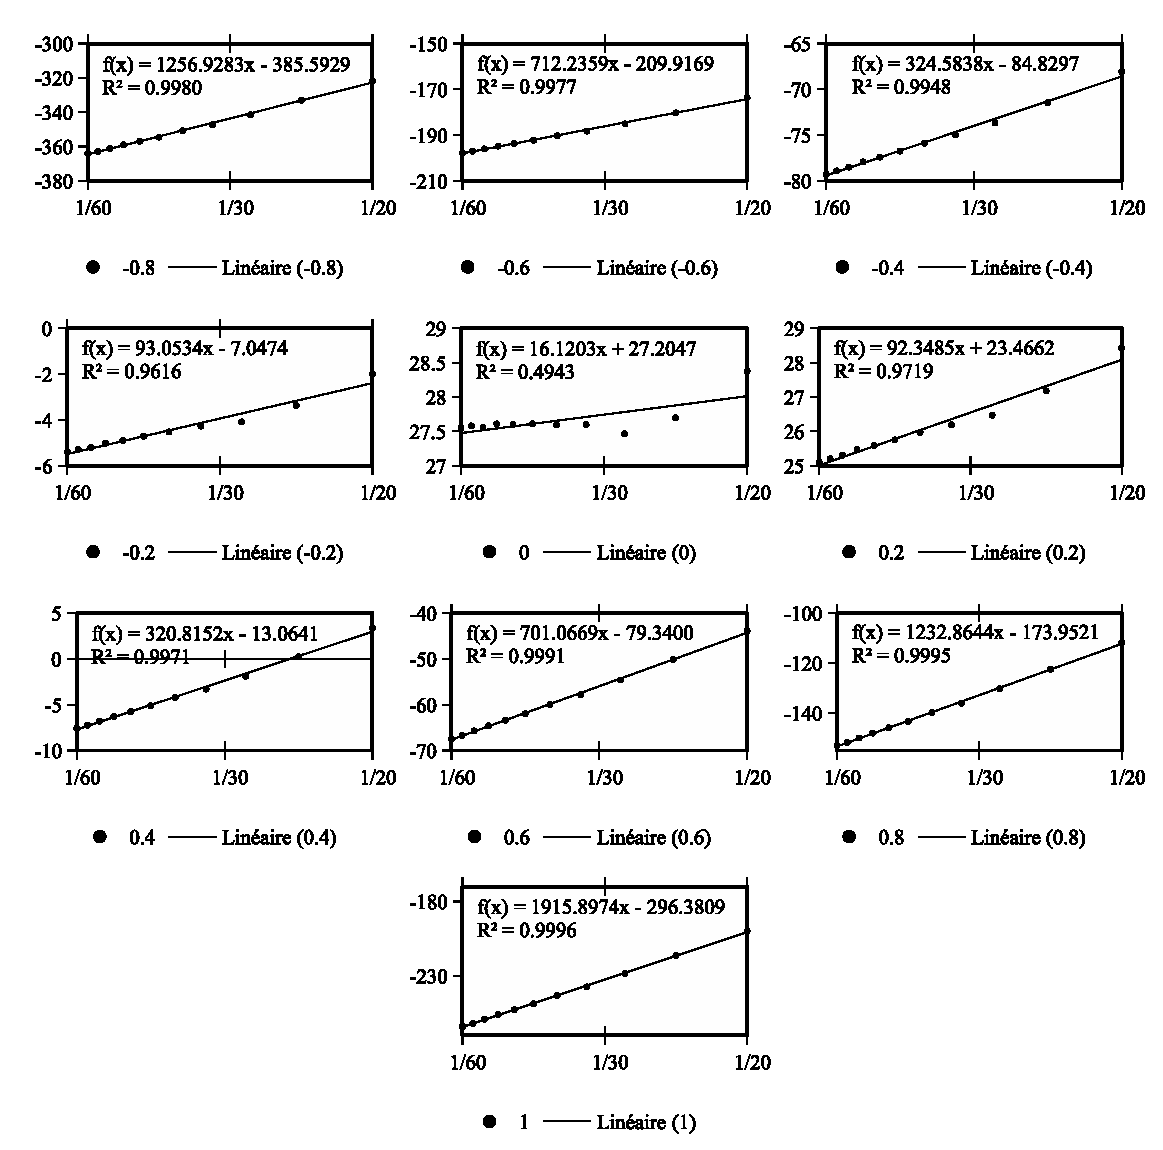
\includegraphics[width=0.95\columnwidth]{_figure/results/ch4_nmax1_lmn}
\par\end{centering}
\caption{Free energy (without correction) of charged $\mathrm{C}\mathrm{H}_{4}$
centre (-1.0 to 1.0) with respect to the box length, for \texttt{\textbf{naive\_nmax1}}
method, with $m_{\max}=n_{\max}=1$, at 300K.\label{fig:ch4_nmax1_lmn}}
\end{figure}

\begin{figure}[!th]
\begin{centering}
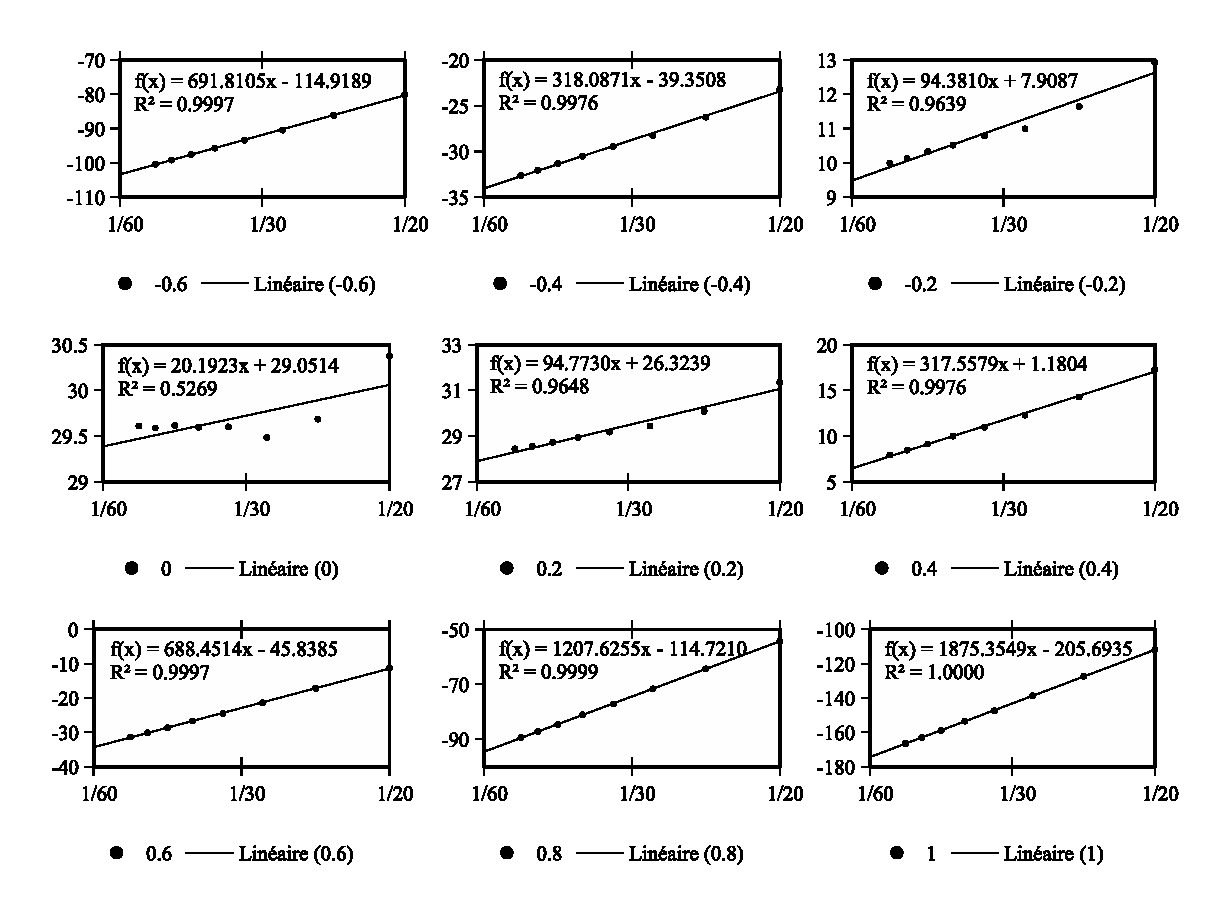
\includegraphics[width=0.95\columnwidth]{_figure/results/ch4_nmax5_inter}
\par\end{centering}
\caption{Free energy (without correction) of charged $\mathrm{C}\mathrm{H}_{4}$
centre (-1.0 to 1.0) with respect to the box length, for \texttt{\textbf{naive\_interpolation}}
method, with 14 angles of Lebedev quadrature angles for $\Theta$
and $\Phi$, 3 for $\Psi$, DCF of $n_{\max}=5$, at 300K.\label{fig:ch4_nmax5_inter}}
\end{figure}

\begin{figure}[!bh]
\begin{centering}
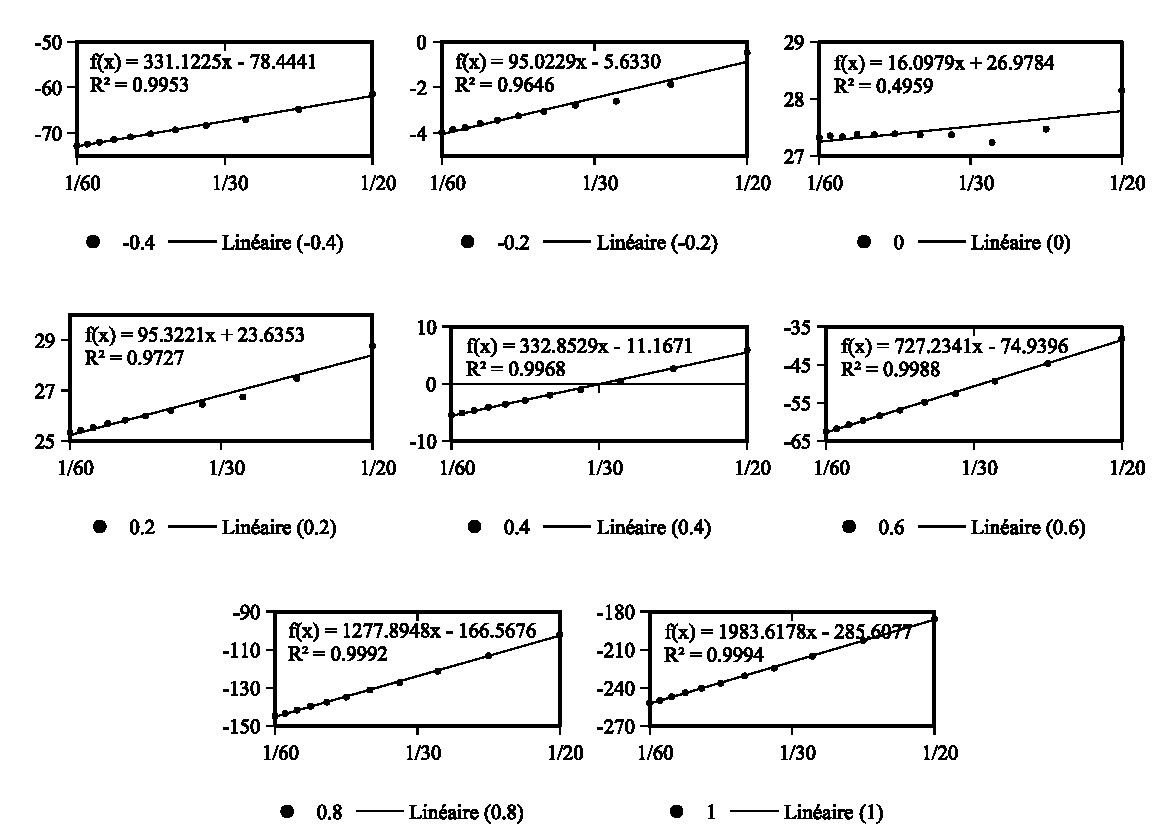
\includegraphics[width=0.95\columnwidth]{_figure/results/ch4_nmax1_new}
\par\end{centering}
\caption{Free energy (without correction) of charged $\mathrm{C}\mathrm{H}_{4}$
centre (-1.0 to 1.0) with respect to the box length, for \texttt{\textbf{convolution\_standard}}
method, with $m_{\max}=n_{\max}=1$, at 298.15K.\label{fig:ch4_nmax1_new}}
\end{figure}

